\chapter{Group Role}
This section describes the multi-group project setting and defines the role of our group’s work in the multi-group project.


The multi-group project consists of several components, including user management, outdoor location based services, and database groups as seen in Figure \ref{fig:astepGroups}.
OD and ID in the figure are abbreviations of respectively outdoor and indoor location based services.
Each group is assigned to one component, and some components have multiple groups assigned to them, and the component architecture can be seen in Figure \ref{fig:astepCore}.


\begin{figure}[h!]
	\centering
	\begin{subfigure}[b]{0.48\textwidth}
		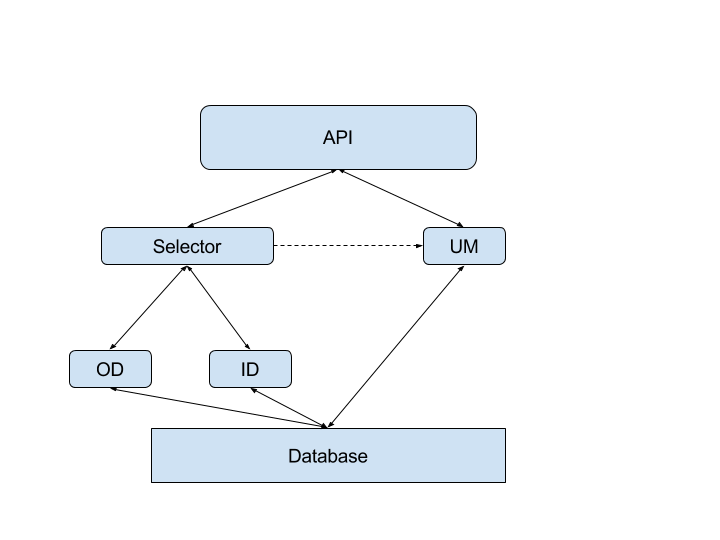
\includegraphics[width=\textwidth]{figures/InformalArchitecture.png}
		\caption{The \gls{astep} core architecture \cite{astepArchitectureImage}. }
		\label{fig:astepCore}
	\end{subfigure}
	~ %add desired spacing between images, e. g. ~, \quad, \qquad, \hfill etc. 
	%(or a blank line to force the subfigure onto a new line)
	\begin{subfigure}[b]{0.48\textwidth}
		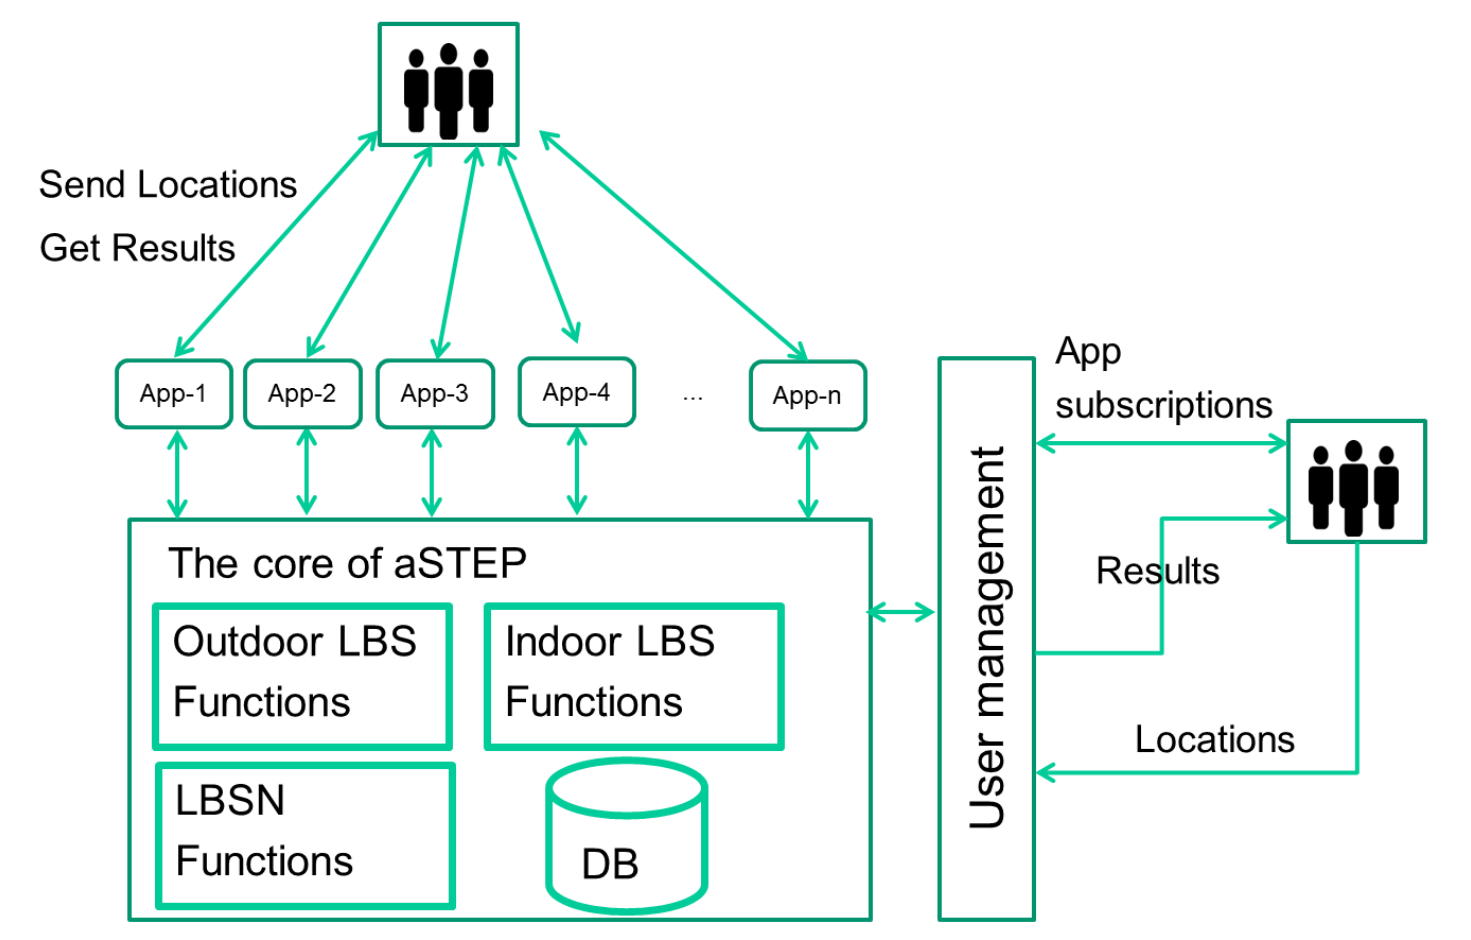
\includegraphics[width=\textwidth]{figures/astepGroups.png}
		\caption{The \gls{astep} group distribution according to the project guidelines.}
		\label{fig:astepGroups}
	\end{subfigure}
	\caption{\gls{astep} architectural design}
	\label{fig:astepArchitecture}
\end{figure}


Our project group is responsible for developing an app that utilizes the \gls{astep} core, and contribute to the development of the interface of the core.
As the project focus is on commuting, the solution will depend upon outdoor location based services.
Any user registration, login or other user related tasks should be handled by the user management group.
According to our project focus and the component architecture, represented in Figure \ref{fig:astepCore}, we will mainly cooperate with the OD and user management groups.